%! Author = kyoto
%! Date = 08.03.2022


\section{Задание}
По выданному преподавателем варианту разработать программу асинхронного обмена данными с внешним устройством. При помощи
программы осуществить ввод или вывод информации, используя в качестве подтверждения данных сигнал (кнопку) готовности ВУ.


\begin{figure}[H]
    \centering
    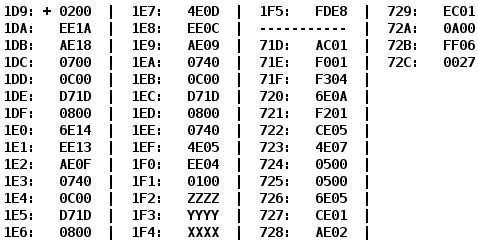
\includegraphics[scale=0.35]{img/variant}
\end{figure}


\section{Программа}

\subsection{Assembler}

\begin{center}
    \begin{tabular}{c}
        \begin{lstlisting}[basicstyle=\ttfamily]
        ORG     0x360
ADDR:	WORD	0x5A1
LEN:	WORD	0x0000
FIRST:	WORD	0x0000
SECOND: WORD    0x0000
START:  LD      (ADDR)+
        AND     #0xFF
        ST      LEN
L:      IN      7
        AND     #0x40
        BEQ     L
        LD      LEN
        OUT     6
BEGIN:	CLA
        LD      (ADDR)+
        ST      SECOND
        SWAB
        ST      FIRST
S1:     IN      7
        AND     #0x40
        BEQ     S1
        LD      FIRST
        AND     #0xFF
        OUT     6
S2:     IN      7
        AND     #0x40
        BEQ     S2
        LD      SECOND
        AND     #0xFF
        OUT     6
        LOOP    LEN
        JUMP    BEGIN
STOP:	HLT

        \end{lstlisting}
    \end{tabular}
\end{center}

\newpage

\subsection{Основная:}
\begin{center}
    \begin{tabular}{|c|c|c|l|}
        \hline
        \textbf{Cell Address} & \textbf{Cell Content} & \textbf{Mnemonics} & \textbf{Comments}                                   \\
        \hline
        360                   & 05A1                  & ADDR               & Текущий адрес ячейки строки.                        \\
        361                   & 0000                  & LEN                & Длина строки + итератор.                            \\
        362                   & 0000                  & FIRST              & Переменная для хранения младшего байта слова.       \\
        363                   & 0000                  & SECOND             & Переменная для хранения старшего байта слова.       \\
        \hline
        364                   & +AAFB                 & LD (-5)+           & Загрузка в аккумулятор длины строки с               \\
        &                       &                    & постинкрементом адреса ячейки.                      \\
        365                   & 2FFF                  & AND \#0xFF         & Выделение значащих младших 8 бит.                   \\
        366                   & EEFA                  & ST (IP-6)          & Сохранение длины строки в ячейку итератора.         \\
        367                   & 1207                  & IN 7               & Считывание SR.                                      \\
        368                   & 2F40                  & AND #0x40          & Проверка 6го бита на "1".                           \\
        369                   & F0FD                  & BEQ (-3)           & Возвращает на считывание SR, если кнопка            \\
        &                       &                    & "Готов" не инициализирована.                        \\
        36A                   & AEF6                  & LD (IP-10)         & Загрузка LEN в аккумулятор                          \\
        36B                   & 1306                  & OUT 6              & Вывод значения аккумулятора в DR.                   \\
        \hline
        36C                   & 0200                  & CLA                & Очистка аккумулятора.                               \\
        36D                   & AAF1                  & LD (-15)+          & Загрузка в аккумулятор текущей ячейки               \\
        &                       &                    & массива с постинкрементом.                          \\
        36E                   & EEF3                  & ST (IP-13)         & Сохранение старшего символа в FIRST.                \\
        36F                   & 0680                  & SWAB               & Обмен байтами.                                      \\
        370                   & EEF0                  & ST (-16)           & Сохраненение младшего слова в SECOND.               \\
        \hline
        371                   & 1207                  & IN 7               & Считывание SR.                                      \\
        372                   & 2F40                  & AND \#0x40         & Проверка 6го бита на "1".                           \\
        373                   & F0FD                  & BEQ (-3)           & Возвращает на считывание SR, если кнопка            \\
        &                       &                    & "Готов" не инициализирована.                        \\
        374                   & AEEC                  & LD (IP-20)         & Загрузка в аккумулятор старшее слово.               \\
        375                   & 2FFF                  & AND \#0xFF         & Выделение младшего байта у загруженного значения.   \\
        376                   & 1306                  & OUT 6              & Вывод значения аккумулятора в DR.                   \\
        \hline
        377                   & 1207                  & IN 7               & Считывание SR.                                      \\
        378                   & 2F40                  & AND \#0x40         & Проверка 6го бита на "1".                           \\
        379                   & F0FD                  & BEQ (IP-3)         & Возвращает на считывание SR, если кнопка            \\
        &                       &                    & "Готов" не инициализирована.                        \\
        37A                   & AEE7                  & LD (IP-33)         & Загружает в аккумулятор младшее слово.              \\
        37B                   & 2FFF                  & AND \#0xFF         & Выделение младшего байта у значения в аккумуляторе. \\
        37C                   & 1306                  & OUT 6              & Вывод значения в DR.                                \\
        37D                   & 8EE2                  & LOOP (IP-38)       & LEN-1, проверка, что LEN $\geqslant$ 0.             \\
        37E                   & CEED                  & JUMP (IP-19)       & Возвращение на начало цикла (в 367).                \\
        37F                   & 0100                  & HLT                & Остановка.                                          \\
        \hline

    \end{tabular}
\end{center}

\subsection{Описание программы:}
Вывод текста сохранённого в массиве в формате АДР0: ДЛИНА АДР1: СИМВ2 СИМВ1 АДР2: СИМВ4 СИМВ3 ... \\
\footnotesize (выводит сначала количество символов, а потом символы в порядке возрастания: СИМВ1, СИМВ2, СИМВ3)\\
\normalsize

\section{Область представления данных и область допустимых значений}

\subsection{Область представления:}
\noindentВ ячейке 360 беззнаковое 11тиразрядное 16теричное число (адрес ячейки).   \\
В ячейках 362-363 символ строки в кодировке ISO-8859-5. \\
В ячейке 361, 5A1 беззнаковое 8миразрядное 16теричное число.    \\
В дальнейших ячейках массива - беззнаковые 16теричные числа, с закодированными символами в младшем и старшем байте. \\

\newpage

\subsection{ОДЗ}

\subsubsection{ADDR:}
\begin{equation*}
    \begin{center}
        $0 \leqslant ADDR \leqslant 2047$\\
    \end{center}
\end{equation*}

\subsubsection{LEN:}
\begin{equation*}
    \begin{center}
        $0 \leqslant LEN \leqslant 2047$\\
    \end{center}
\end{equation*}

\subsubsection{$M_i$:}
\begin{equation*}
    \begin{center}
        $20_{16} \leqslant $M_{i}$ \leqslant FF_{16}$\\
    \end{center}
\end{equation*}


\section{Расположение программы в памяти БЭВМ:}
\noindent\textit{Программы - \textbf{360-37A} . \\
Выводимая строка – \textbf{5A1-(5A1+LEN-1)} .  \\}
